\subsection{Introducción}
Observamos  $\samples\in\R^d\times\R$ muchos datos (potencialmente infinitos) de dimensión (posiblemente) grande.
\begin{example}[Clasificación de imágenes]
Tenemos un conjunto de imágenes, cada una con una etiqueta. Por ejemplo, la foto de un gato, como se grafica en figura \ref{fig:gato}\footnote{Fuente: \url{https://dongminlee.tistory.com/18}}, puede representarse como un vector al ``aplanar'' la matriz correspondiente a la imagen. Las distintas $k$ clases posibles pueden enumerarse de modo que al concepto \textit{gato} se le asigna un número $y\in\{1,\dots,k\}\subset\N\subset\R$.
\begin{figure}
    \centering
    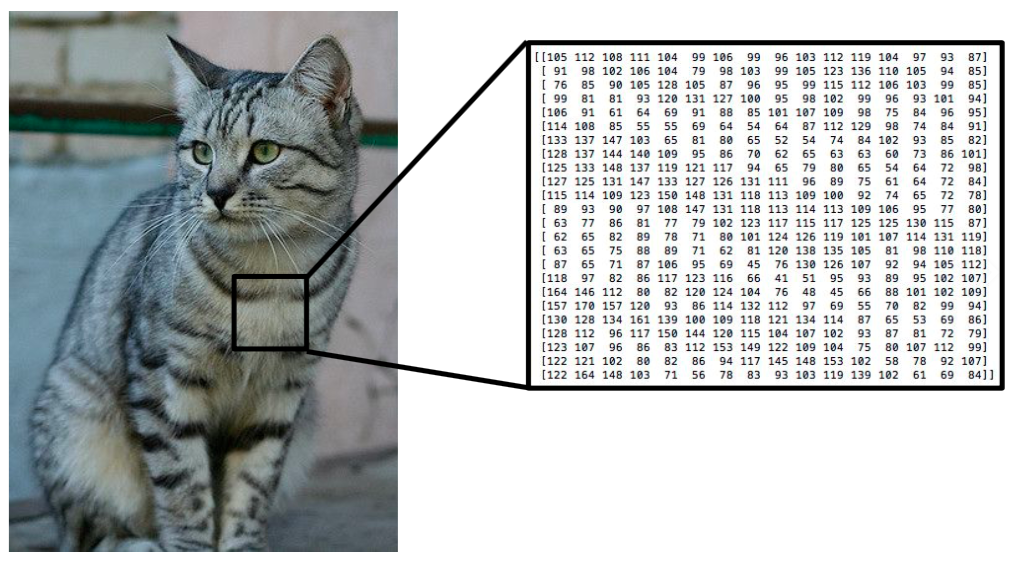
\includegraphics[scale=0.32]{img/figura_gato.png}
    \caption{Imagen con etiqueta ``gato''.}
    \label{fig:gato}
\end{figure}
De este modo, dado un elemento $i$ de nuestros $n$ datos, $x_i\in\R^d$ es un vector que representa la imagen, mientras que $y\in\{1,\dots,k\}$ corresponde a una etiqueta.
\end{example}
\newp \textbf{Objetivo}: aprender de los datos, i.e., aprender a predecir, al ver un $x$ nuevo, la etiqueta $y$ correspondiente.
\begin{example}[Redes Neuronales]
\label{ejemplo:red_neuronal}
Se busca predecir $y$ mediante
% $$ \hat{y}(x,\theta) = \displaystyle \frac{1}{N}\sum^N_{j=1}\sigma_*(x_j,b_j) \,.$$
$$ \hat{y}(x,\theta) = \displaystyle\sum^N_{j=1}\sigma_*(x_j,\theta_j) \,.$$
donde:
\begin{itemize}
    % \item $\sigma_*:\R^d\times\R^D\to\R$ se llama función de activación.
    \item $N$ es el número de neuronas.
    \item $\theta=(\theta_1,\dots,\theta_N)\in(\R^D)^N$ son los parámetros (``pesos'').
    \newline En general, para $j=1,\dots,N$ tomamos $\theta_j=(a_j,b_j,\omega_j)\in \R\times\R\times\R^D $ y $\sigma_*$ de la forma
    $$ \sigma_*(x,\theta_j)=a_i\sigma(\langle x,\omega_i\rangle+b_i) \,.$$
\end{itemize}
\textbf{¿Como aprende?}
\begin{itemize}
    \item Consideramos $l:\R\times\R\to\R_+$ función de pérdida.
    \newline Ej: $l(y,\hat{y})=(y-\hat{y})^2$
    \item Idealmente, buscamos
    $$ \hat{\theta}=\displaystyle\arg\min_\theta \sum^M_{i=1}l(y_i,\hat{y}(x_i,\theta))\,,$$
    con $M$ grande.
    \item Primera idea: aplicar un algoritmo de optimización para ``entrenar la red'' con los datos conocidos. Es decir, encontrar $\hat{\theta}$ óptimo (o casi).
\end{itemize}
\textbf{Problemas}:
\begin{itemize}
    \item Función objetivo costosa de evaluar, debido a una o varias de las razones siguientes:
    \begin{itemize}
        \item $M$ es grande
        \item $d$ es grande, donde $d$ es la dimensión de $x_i$.
        \item $N$ es grande
    \end{itemize}
    \item Requiere tiempo y memoria computacionales (se requiere usar toda la información en todos los pasos).
    \item Sobreajuste (overfitting): Si entrenamos ``perfectamente'' usando todos los $\samples$ (mínimo global) sobreajustamos y perdemos la ``capacidad de generalización''.
\end{itemize}
\textbf{Segunda idea}: Supongamos $(x_i,y_i)\sim\iid$ de ley $\mu$ no conocida.
\newline En vez de buscar
\begin{alignat*}{2}
        \hat{\theta} & = \displaystyle\arg\min_\theta\sum^M_{i=1}l(y_i,\hat{y}(x_i,\theta)) \\
         & = \arg\min_\theta \frac{1}{M}\sum^M_{i=1}l(y_i,\hat{y}(x_i,\theta), 
    \end{alignat*}
buscamos
$$ \hat{\theta}=\displaystyle\arg\min_\theta \E(l(y,\hat{y}(X,\theta)))$$
con $(X,Y)\sim\mu$.
\newp \textbf{¿Tiene sentido?, ¿de qué sirve si no conocemos $\mu$? ¿qué cambia?}
\end{example}
\vspace{1cm}\\
\subsection{Algoritmo de gradiente estocástico}
El descenso de gradiente estocástico (o \textit{S.G.D.} por sus siglas en inglés) es uno de los pilares del desarrollo reciente del aprendizaje de máquinas y de la inteligencia artificial.
\newp Bibliografía: \textit{Stochastic Approximation} (Robbins \& Monro) \cite{robbins}...... Referencia m\'as actual: \textit{Online Learning and Stochastic Approximations} \cite{bottou}.

\subsubsection{El algoritmo}
Consideramos el problema
$$ \min_\theta \E(f(\theta,X)) \, ,$$
con:
\begin{itemize}
\item $f:\R^d\times \R^k\to\R$
    \item $X\sim\mu$
    \item $(\gamma_t)_{t\in\N}$ pasos o tasa de aprendizaje (\textit{learning rate})
\end{itemize}
 Asumiremos en lo que sigue que $f$ es tal que $F(\theta):= \E(f(\theta,X))$ est\'a bien definida, y que se cumple la relaci\'on $\nabla F(\theta)=\E(\nabla_\theta f(\theta,X)) $ para todo $\theta$.
 
En vez de usar un algoritmo gradiente usual $\theta^{t+1}=\theta^t-\gamma_{t+1}\nabla F(\theta^t)=\theta^t-\gamma_{t+1}\E(\nabla_\theta f(\theta^t,X))$, con $(\gamma_t)_{t\in\N}$ sucesión en $\R_+$ pasos, la idea ser\'a \textbf{considerar observaciones} $x_1,x_2,\dots,x_t \iid \sim\mu$ y el algoritmo definido por las iteraciones: 
$$ \theta^{t+1}:=\theta^t-\gamma_{t+1}\nabla_\theta f(\theta^t,x_{t+1})\,.$$
\begin{remark}
\beforeitemize
\begin{itemize}
    \item El término $\nabla_\theta f(\theta^t,x_{t+1})$ se puede ver como un gradiente exacto perturbado por cierto ruido aleatorio, m\'as precisamente, 
    $$ \nabla_\theta f(\theta^t,x_{t+1})=\E(\nabla_\theta f(\theta^t,X))+\Delta_{t+1}=\nabla F(\theta^t)+\Delta_{t+1},$$
    con $\Delta_{t+1}=\nabla_\theta f(\theta^t,x_{t+1})-\E(\nabla_\theta f(\theta^t,X))$  v.a. centrada. 
    \item En cada paso necesitamos evaluar una sola vez $\nabla_\theta f$ (en un solo dato nuevo).
    \item Podemos usar los datos a medida que llegan.
    \item \textbf{Caso particular importante (literatura de optimización)}
    \newline Se quiere optimizar $\tilde{F}(\theta):=\displaystyle\sum^M_{i=1}\tilde{f}_i(\theta)$, con $\tilde{f}_i:\R^d\to\R$ ($M$ funciones), lo cual es equivalente a
    % \newline $\ssi$ 
    optimizar $F(\theta)=\displaystyle\frac{1}{M}\sum^n_{i=1}\tilde{f}_i(\theta)=\E(f(I,\theta))$ con $I=X\sim \frac{1}{M}\sum^M_{i=1}\delta_i$ (esto es,  $I\in\{1,\dots,M\}$ es un índice  aleatorio  elegido de manera uniforme), y $f(i,\theta)=\tilde{f}_i(\theta)$.  Entonces, 
    $$ \theta^{t+1}:=\theta^t-\gamma_t \nabla_\theta f(\theta^t,I_{t+1})=\theta^t-\gamma_t \nabla_\theta\tilde{f}_{I_{t+1}}(\theta), $$
    con $I_1,I_2,\dots \iid\sim\mathbb{U}(\{1,\dots,M\})$.
\end{itemize}
\end{remark}
El siguiente es un enunciado cl\'asico sobre este tipo de algoritmo, que damos inicialmente sin todos los detalles: 
\begin{theorem}[Sigmund, Robbins, (1951)] 
Bajo hipótesis razonables sobre $f$ (regularidad en $\theta$, integrabilidad de $\nabla_\theta f_+$, cotas), si $\gamma_t\,\substack{\searrow \\ \tiny{t\to\infty}}\, 0$ suficientemente lento la sucesión:
$$ \theta^t\mbox{ }\overset{c.s.}{\substack{\longrightarrow \\t \to \infty}}\mbox{ }\mbox{ Conjunto de puntos críticos de } F(\theta)=\E(f(\theta,X)).$$
Más aún, si $f$ es convexa,  estrictamente en $\theta$ (más algunas hipótesis adicionales), entonces
$$ \theta^t\mbox{ }\overset{c.s.}{\substack{\longrightarrow \\t \to \infty}}\mbox{ }\arg\min_\theta \E(f(\theta,X))\,.$$
\end{theorem}
\begin{remark}

Si bien este tipo de resultados fueron obtenidos por primera vez hace cerca de 70 años, la utilizaci\'on del descenso de gradiente estocástico (o \textit{S.G.D.}  ha sido fuertemente reimpulsada con el desarrollo reciente  del aprendizaje de máquinas y de la inteligencia artificial pues, entre otros motivos, los siguientes: 
\begin{itemize}
    \item Permite ``entrenar'' (estimar) parámetros con datos,  a medida que estos  van llegando.
    \item Permite ``actualizar'' la estimación en tiempo real (a medida que llegan nuevos datos).
    \item Es ``escalable'': el costo es temporal (uso de memoria constante) y proporcional al tamaño del conjunto de datos.
    \item Si bien no está garantizada la convergencia a un óptimo global, muchas veces permite encontrar un mínimo local $\hat{\theta}=\theta^t$ que ``generaliza bien'' (como estimador) en el sentido siguiente:  si $t$ es suficientemente grande,  $X_1,\dots,X_t$ es el conjunto de entrenamiento,  y  $X_{t+i}, i=0,\dots, N$ son datos nuevos,  entonces
    $$ \displaystyle\frac{1}{N}\sum^N_{i=1}f(\theta^t,X_{t+i})\mbox{ es cercano a }\E(f(\theta^t,X)) \mbox{ y } \E(f(\theta^t,X)) \mbox{ es cercano a } \min_\theta \E(f(\theta,X)). $$
\end{itemize}
\end{remark}
   
\begin{remark} Desde el punto de vista pr\'actico: 
\begin{itemize}
\item Típicamente, se buscan mínimos locales ``buenos'', de valores cercanos al global, pero no necesariamente un m\'inimo global.
    \item Se sugiere correr el algoritmo desde muchos $\theta_0$ iniciales y guardar el mejor valor obtenido.
    \item Se sugiere probar adem\'as distintas elecciones de paso $\gamma_t$ y guardar la que de mejores resultados. En la práctica se suele usar $\gamma_t=$constante o constante por tramos ($t$ no tiende a infinito en la vida real)
    \item Hay muchas variantes para acelerar ``convergencia'' o bien para explorar mejor el espacio. Un ejemplo de eso \'ultimo es agregar ``ruido'' o aleatoriedad adicional,  para evitar quedar atrapado en  mínimos locales malos.
    \end{itemize}
\end{remark}
\begin{notation}
En lo que sigue, denotamos $\partial f(\theta,x)=\nabla_\theta\,.
\end{notation}
\subsubsection{Convergencia en el caso convexo}

Para probar la convergencia en el caso convexo necesitaremos herramientas de cálculo estocástico.
\begin{definition}[Martingala]
Sea $(\Omega,\mathcal{F},\P)$ un espacio de probabilidad dotado de una filtración $(\mathcal{F}_t)_{t\in\N}$ (i.e., $\sigma$-álgebras tal que $\forall t\in\N$, $\mathcal{F}_t\subset\mathcal{F}_{t+1}\subset\mathcal{F}$).  Una familia de variables aleatorias se dice martingala si
$$ X_t\in L^1(\mathcal{F}_t) \forall t\in\N$$ y $$\forall t\in\N\espacio \E(X_{t+1}|\mathcal{F}_t)=X_t  \mbox{ c.s.}$$
\begin{notation}
Si en la última ecuación tenemos $\geq$ en vez de igualdad entonces la familia se dice \textbf{sub-martingala}. Si tenemos $\leq$ entonces la llamamos \textbf{sobre-martingala}.
\end{notation}
\end{definition}
En particular usaremos el siguiente teorema del curso de cálculo estocástico, que asumiremos sin demostración.
\begin{theorem}[Convergencia sobre-martingalas]
\label{theorem:sobre-m}
Sea $(X_t)_{t\in\N}$ una sobre-martingala con respecto a $(\mathcal{F}_t)_{t\in\N}$ tal que $\displaystyle\sup_{t\in\N}\E(X_t^-)<\infty$. Entonces $\exists X_\infty\in L^1$ tal que $$ X_t\convcst X_\infty \,.$$
\end{theorem}
\begin{theorem}[Descenso de gradiente estocástico caso convexo]
\label{teo:sgd}
Supongamos que los datos ....  son v.a. i.i.d. de ley $\mu$ definas en un espacio de probabilidad $(\Omega,\mathcal{F},\P)$.  Adem\ás, supongamos que:  
\begin{itemize}
    \item[i)] $\forall \theta\, , f(\theta,\cdot)\in L^1(\mu). \mbox{ Adem\'as }  $f(\cdot,x)\in\mathcal{C}^1 \mu(dx)-c.s.$,  \mbox{ y } $\partial_\theta f(\theta,\cdot)\in L^1(\mu)$
    \item[ii)] $F$ tiene un único mínimo $\theta^*$
    \item[iii)] $\forall \epsilon >0$, $\displaystyle \inf_{\theta:\|\theta-\theta^*\|^2>\epsilon}(\theta-\theta^*)\nabla F(\theta)>0$
    \newline i.e., lejos de $\theta^*$, $F$ decrece estrictamente, uniformemente hacia $F(\theta^* )$
    \item[iv)] $\exists A,B\geq 0$ tal que $\E(\|\partial f(\theta,X)\|^2)\leq A+B\|\theta-\theta^*\|^2, \forall \theta$
    \item[v)] $\sum_{t\in\N}\gamma_t=\infty$, $\sum_{t\in\N}\gamma_t^2<\infty$ \espacio (por ejemplo: $\gamma_t=\frac{1}{t}$).
\end{itemize}
Entonces
$$ \theta_t\mbox{ }\overset{c.s.}{\substack{\longrightarrow \\t \to \infty}}\mbox{ }\theta^*\,.$$

\end{theorem}
\begin{remark}
\beforeitemize
\begin{itemize}
\item (i) $\implies F\in\mathcal{C}^1(\R^d)$ con  $\nabla F=\E(\partial_\theta f(\theta,x))$. 
     \item Si bien no pedimos explícitamente que la función $F$ sea  convexa, haciendo un Taylor en $\theta$ se puede verificar que las hipótesis ii) y iii) se cumplen, si  $F$ es  de clase ${\cal C}^2$ y estrictamente convexa. 
     \item (iii)  impide que el gradiente se ``aplane'' lejos del m\'inimo global. 
    \item (iv) se cumple si por ejemplo $f(\cdot,x)$ es  de clase ${\cal C}^2$ con  $\E(\|Hess_\theta f(\theta,X)\|)<\infty$ % . TERMINAR LA REMARK
\end{itemize}
\end{remark}
\begin{proof}[Demostración de Teorema \ref{teo:sgd} descenso de gradiente estocástico, caso convexo]
\gris \\ Tomemos la función  siguiente como “funci\'on de de Lyapunov" :
$$ h(\theta) = \|\theta-\theta^*\|^2\, , $$
y denotemos $h_t:=h(\theta_t)$. Queremos probar que $h_t$ converge a $0$ c.s., con lo cual tendremos que $\theta_t\mbox{ }\overset{c.s.}{\substack{\longrightarrow \\t \to \infty}}\mbox{ }\theta^*$. En efecto,
$$ \theta_{t+1}-\theta^* = \theta_t-\theta^*-\gamma_t\partial f(\theta_t,x_{t+1}) \,.$$
Luego aplicando $\|\espacio\|^2$,
$$ \|\theta_{t+1}-\theta^*\|^2 = \|\theta_t-\theta^*\|^2-2\gamma_t(\theta_t-\theta^*)\partial f(\theta_{t},x_{t+1})+\gamma^2_t\|\partial f(\theta_t,x_{t+1})\|^2 \,,$$
entonces
$$ h_{t+1}-h_t = -2\gamma_t(\theta_t-\theta^*)\partial f(\theta_t,x_{t+1})+\gamma_t^2\|\partial f(\theta_t,x_{t+1})\|^2 \, .$$
Ahora haremos aparecer una sobre-martingala. Tomemos como filtración la tribu generada por las observaciones, i.e.,$ (\mathcal{F}_t=\sigma(x_0,\dots,x_t))_{t\in\N}$, asumiendo adem\'as que la condici\'on inicial $\theta_0$ es determinista. 

Por inducci\'on se ve f\'acilmente  que  $\theta_t\in L^2(\Omega,\mathcal{F},\P)\,\forall t\in\N$, gracias a la condici\'on iv). Tomando esperanza condicional respecto a $\mathcal{F}_t$:
$$ \E(h_{t+1}-h_t|\mathcal{F}_t)  = -2\gamma_t(\theta_t-\theta^*)\E(\partial f(\theta,X))\big\vert_{\theta = \theta_t}  +\gamma_t^2\E(\|\partial f(\theta,X)\|^2)\big\vert_{\theta = \theta_t} \,,$$
donde usamos que $x_{t+1}\indep \mathcal{F}_t$, con lo cual $\E( G(\theta_t,x_{t+1})|\mathcal{F}_t)) = \E(G(\theta,X))\vert_{\theta = \theta_t}$ para toda $G$ apropiada. Además, por (iv),  $\exists A,B\geq 0$ tal que $\E(\|\partial f(\theta,X)\|^2)\big\vert_{\theta = \theta_t} \leq A+B\|\theta_t-\theta^*\|^2$, por ende
$$ \E(h_{t+1}-h_t|\mathcal{F}_t) \leq -2\gamma_t(\theta-\theta^*)\E(\partial f(\theta,X))\big\vert_{\theta=\theta_t} +A\gamma_t^2+B\gamma_t^2 h_t \,.$$
Como $h_t$ es $\mathcal{F}_t$-medible, puede entrar en la esperanza condicional del lado izquierdo, con lo cual 
\begin{alignat*}{2}
\E(h_{t+1}-(1+\gamma_t^2 B)h_t|\mathcal{F}_t) & \, \leq \, -2\gamma_t(\theta_t-\theta^*)\nabla F(\theta_t)+\gamma_t^2 A .
\end{alignat*}
 Definimos $\mu_t:=\displaystyle\prod^{t-1}_{k=1}\frac{1}{1+\gamma_k^2B}$ y $h'_t:=\mu_th_t$. Multiplicando por $\mu_{t+1}$ queda que
$$ \E(h'_{t+1}-h_t'|\mathcal{F}_t)\leq -2\gamma_t(\theta_t-\theta^*)\nabla F(\theta_t) + \gamma_t^2A\mu_{t+1}   \, \leq \gamma_t^2A\mu_{t} \,,   $$
donde usamos (iii) y el hecho que $\mu_{t+1}\leq \mu_t $. Notar que $\mu_t \convt \mu_\infty\in(0,\infty)$, como puede verse tomando logaritmo y usando que $\sum\gamma_t^2<\infty$. De la desigualdad anterior deducimos que
$$ X_t:=h_t'-\displaystyle\sum^{t-1}_{k=0}A\gamma_t^2\mu_t$$
es una sobre-martingala con respecto a $(\mathcal{F}_t)_{t\in\N}$, es decir $\E(X_{t+1}|\mathcal{F}_t)\leq X_t\,\forall t\in\N$. Para usar el Teorema \ref{theorem:sobre-m} de convergencia de  sobre-martingalas, veamos que es acotada por debajo. En efecto, como $h_t'\geq 0$, tenemos que 
$$ X_t \geq 0 - \displaystyle A\sum^\infty_{k=0}\gamma_t^2\cdot(\sup_{j\in\N}\mu_j)>-\infty.  $$
Así, por el Teorema de convergencia de  sobre-martingalas, 
 $\exists X_\infty\in L^1$ tal que $X_t\convcst X_\infty$. Dado que 
 $$A\sum^N_{t=1}\gamma_t^2\mu_t \mbox{ }\substack{\longrightarrow \\ N\to\infty}\mbox{ } A\sum^\infty_{t=1}\gamma_t^2\mu_t <\infty, $$ se sigue que
$ h'_t \mbox{ }\overset{c.s.}{\substack{\longrightarrow \\t \to \infty}}\mbox{ } h'_\infty \,,$
para cierta v.a. $ h'_\infty\in L^1$, 
y puesto que $\mu_t \convt \mu_0\in(0,\infty)$, deducimos que $$h_t\mbox{ }\overset{c.s.}{\substack{\longrightarrow \\t \to \infty}}\mbox{ }h_\infty$$ para cierta $h_\infty\in L^1$. 
Para concluir el teorema,  veamos que $h_\infty=0\,c.s.$.  Volviendo a la desigualada satisfecha por $\E(h'_{t+1}-h_t'|\mathcal{F}_t)$, vemos que 
$$ 0\leq 2\mu_t \gamma_t(\theta_t-\theta^*)\nabla F(\theta_t)\leq \gamma_t^2A\mu_t + \E(h'_t-h'_{t+1}|\mathcal{F}_t) \,,$$
de donde
\begin{alignat*}{2}
 2\E(\displaystyle\sum^N_{t=0}\gamma_t\mu_t(\theta_t-\theta^*)\nabla F(\theta_t)) & \leq \displaystyle\sum^N_{t=1}\gamma_t^2 A\mu_t+\E(h_0)-\E(h_{N}) \\
& \leq A\sum^{\infty}_{t=1}\gamma_t^2\mu_t+\E(h_0)<+\infty
\end{alignat*}
$$ \therefore \espacio \displaystyle\sum^\infty_{t=0}\gamma_t\mu_t(\theta_t-\theta^*)\nabla F(\theta_t)<\infty \espacio c.s.\,.$$
Puesto que $\mu_t\convt\mu_\infty\in(0,\infty)$, $\mu_t$ est\'a acotada por debajo lejos de $0$, por lo que 
$$  \displaystyle\sum_t\gamma_t(\theta_t-\theta^*)\nabla F(\theta_t)<\infty \, c.s.\,.$$
Usando (v),\espacio $\displaystyle\sum_t\gamma_t=\infty$, con lo cual necesariamente se cumple que 
$$ \displaystyle\liminf_{t\to\infty}(\theta_t-\theta^*)\nabla F(\theta_t) = 0 \,c.s.\,.$$
Para concluir, consideremos $\Omega'_\epsilon=\{h_\infty>\sqrt{\epsilon}\}$ y supongamos que $\P(\Omega'_\epsilon)>0$. Usando (iii) tenemos que $\P(\displaystyle\liminf_{t\to\infty}(\theta_t-\theta^*)\nabla F(\theta_t)>0)\geq \P(\Omega'_{\epsilon/2})  >0$, que es una contradicción. 
$$ \therefore\espacio \P(\Omega'_\epsilon)=0\espacio\forall\epsilon>0,\espacio \Longrightarrow\espacio h_\infty=0\espacio c.s.\,. $$ \findem
\negro
\end{proof}
\vspace{1cm}\\
\subsubsection{Convergencia en caso no-convexo}
\begin{theorem}[Extensión de Descenso de gradiente estocástico (caso no-convexo)]
\label{theorem:sgd_no_conv}
Supongamos:
\begin{itemize}
    \item[i)] $f(\theta,\cdot)\in L^1(\mu)$, $f(\cdot,x)\in\mathcal{C}^3,  \mu(dx)-c.s.$, $\partial^k f(\theta,\cdot)\in L^1(\mu), k=1,2,3$ (luego $F\in\mathcal{C}^3$)
    \item[ii)] $F$ es acotada por debajo
    \item[iii)] $\exists A_k,B_k\geq 0$ tal que $\E(\|\partial f(\theta,X\|^k)\leq A_k+B_k\|\theta\|^2,\espacio k=1,2,3$
    \item[iv)] $\forall M >0$, $\displaystyle \inf_{\theta:\|\theta\|^2>M}\theta\nabla F(\theta)>0$
    \item[v)] $\sum_{t\in\N}\gamma_t=\infty$, $\sum_{t\in\N}\gamma_t^2<\infty$
\end{itemize}
Entonces tenemos lo siguiente (casi seguramente):
\begin{itemize}
    \item[a)] $(\theta_t)_{t\in\N}\subset \mbox{ un compacto }\R^d$
    \item[b)] $\exists F_\infty \in L^1 \mbox{ tal que }F(\theta_t)\convcst0$
    \item[c)] $\nabla F(\theta_t)\convcst 0$
\end{itemize}
\end{theorem}

\begin{remark}
\beforeitemize
\begin{itemize}
    \item El resultado no implica convergencia c.s. de $(\theta_t)_{t\in\N}$\,.
    \item (a)$\implies$ toda subsucesión tiene una subsucesión convergente c.s. $\theta_{t_k}\mbox{ }\substack{\longrightarrow \\ k\to\infty}\mbox{ } \tilde{\theta}$
    \newline (b), (c) $\implies$ por continuidad de $F$ y $\nabla F$,
    $$F(\theta_{t_k})\mbox{ }\substack{\longrightarrow \\ k\to\infty}\mbox{ }F(\tilde{G})\espacio\land\espacio \nabla F(\theta_{t_k})\mbox{ }\overset{c.s.}{\substack{\longrightarrow \\k \to \infty}}\mbox{ }0=\nabla F(\tilde{\theta})\,.$$
    \newline $\therefore\mbox{ si }Crit:\{\theta:\nabla F(\theta)=0\}$, $\forall \epsilon>0$, $\P(dist(\theta_t,Crit)>\epsilon)\mbox{ }\substack{\longrightarrow \\ t\to\infty}\mbox{ }0$\espacio, i.e., la probabilidad de estar a distancia positiva de puntos críticos tiende a $0$.
\end{itemize}
\end{remark}
\vspace{.75cm}\\
\begin{proof}[Esquema de Demostración de Teorema \ref{theorem:sgd_no_conv}, gradiente estocástico, caso no-convexo]
\gris 
% Veremos un esquema de demostración. 
Para más detalles ver Bottou et al. \cite{bottou}.
\newp Usaremos nuevamente el argumento con sobre-martingalas usando una función de Lyapunov ($h(\theta)$). Veremos un confinamiento, o sea que el algoritmo nos llevará a estar en un compacto. Tomamos
$$ h(\theta) = (\|\theta\|^2-M)^2_+=\phi(\|\theta\|^2)\,,$$
donde $\phi(r)=(r-M)_+^2$, y tomamos $h_t:=h(\theta_t)\,\forall t\in\N$. Usando la hipótesis (iii) y un Taylor de orden 1 se demuestra que
$$ \E(h_{t+1}-h_t|\mathcal{F}_t) \leq -2\gamma_t\theta_t\nabla F(\theta_t)\phi'(\|\theta\|^2)+\gamma_t^2(A+Bh_t) \,, $$
con $\phi'(r)=\begin{cases}
0 & r\leq M \\ 2(r-M) & r>M \, .
\end{cases}$ 
\newline Luego por Teorema \ref{theorem:sobre-m}, $h_t\convt h_\infty\in L^1$. Entonces
$$ \displaystyle\sum_{t=0}^\infty\gamma_t\theta_t\nabla F(\theta_t)\phi'(\|\theta_t\|^2)<\infty\espacio c.s. \, , $$
y como por (v) tenemos $\sum\gamma_t=\infty$, necesariamente $\displaystyle\liminf_{t\to\infty} \theta_t\nabla F(\theta_t)\phi'(\|\theta_t\|^2) = 0$. Además, por (iv) $\displaystyle\liminf_{t\to\infty}\phi'(\|\theta_t\|^2)=0\espacio \implies \espacio h_\infty=0\,c.s.\espacio$, $\therefore \|\theta_t\|\leq 2M \espacio c.s.$ para todo $t$ suficientemente grande (aleatorio).
\newp Para demostrar la convergencia de $F(\theta_t)$ usamos un Taylor de orden 1 para obtener 
$$ F(\theta_{t+1})-F(\theta_t)\leq -\gamma_T\partial f(\theta_t,X_{t+1})\nabla F(\theta_t)+\frac{1}{2}\gamma^2_t\|\partial f(\theta_t,X_{t+1})\|^2\partial^2F(\tilde{\theta}_t) \,,$$
luego obtenemos una sobre-martingala al tomar esperanza condicional con respecto a $\mathcal{F}_t$. Luego definiendo $h_t:=F(\theta_t)\espacio(\geq cte)$ se demuestra que
$$ \E(h_{t+1}-h_t|\mathcal{F}_t) \leq -\gamma_t\|\nabla F(\theta_t)\|^2+\gamma_t^2C \,,$$
y nuevamente tenemos que existe $F_\infty\in L^1$ tal que $F(\theta_t)=h_t\convt F_\infty$.

\newp Para la convergencia de $\nabla F(\theta_t)$ a $0$ notemos que
$$ \E(h_{t+1}-h_t|\mathcal{F}_t) \leq -\gamma_t\|\nabla F(\theta_t)\|^2+\gamma_t^2C \espacio \implies \espacio \displaystyle\sum^\infty_{t=1}\gamma_t\|\nabla F(\theta_t)\|^2<\infty \,,$$
con lo cual $\displaystyle\liminf_{t\to\infty}\|\nabla F(\theta_t)\|^2=0$. Para concluir debemos mostrar que $h_t:=\|\nabla F(\theta_t)\|^2$ es convergente. En efecto haciendo un taylor de orden 2 para $\|\nabla F\|^2$ tenemos
$$ \|\nabla F(\theta_{t+1})\|^2-\|\nabla F(\theta_t)\|^2 \leq -2\gamma_t\partial f(\theta,X_{t+1})Hess(F(\theta_t))\nabla F(\theta_t)+\gamma_t^2\|\partial^2 f(\theta,X_{t+1})\| M''' \,,$$
luego
$$ \E(h_{t+1}-h_t|\mathcal{F}_t) \leq 2\gamma_t\|\nabla F(\theta_t)\|^2 +\gamma_t^2M''' \,.$$
Basta notar que tanto $2\gamma_t\|\nabla F(\theta_t)\|^2$ como $\gamma_t^2M'''$ son convergentes, por ende podemos usar nuevamente el Teorema \ref{theorem:sobre-m} para encontrar un $h_\infty$, que necesariamente debe ser $0$ por lo anterior, i.e.,
$$ h_t = \|\nabla F(\theta_t)\|^2\convt 0\,c.s.$$
\findem
\negro
\end{proof}
\begin{remark}[\textbf{Posibilidades a tener en mente}]
% \textbf{Posibilidades a tener en mente}
Al correr el algoritmo podemos encontrarnos en los siguientes casos, graficado en la figura \ref{fig:sgd}.
\begin{itemize}
    \item Mínimo local: Ok, eligiendo el mejor entre muchas corridas.
    \item Máximo local (u otra cosa): Malo, pero fácil de descartar.
    \item Mínimo global: No necesariamente deseable pues se corre el riesgo de sobreajustar. Además es ``inalcanzable''.
    \item Plateau asintótico: Muy malo. No deberia ocurrir bajo la hipótesis (iv).
\end{itemize}
\end{remark}
\begin{figure}
    \centering
    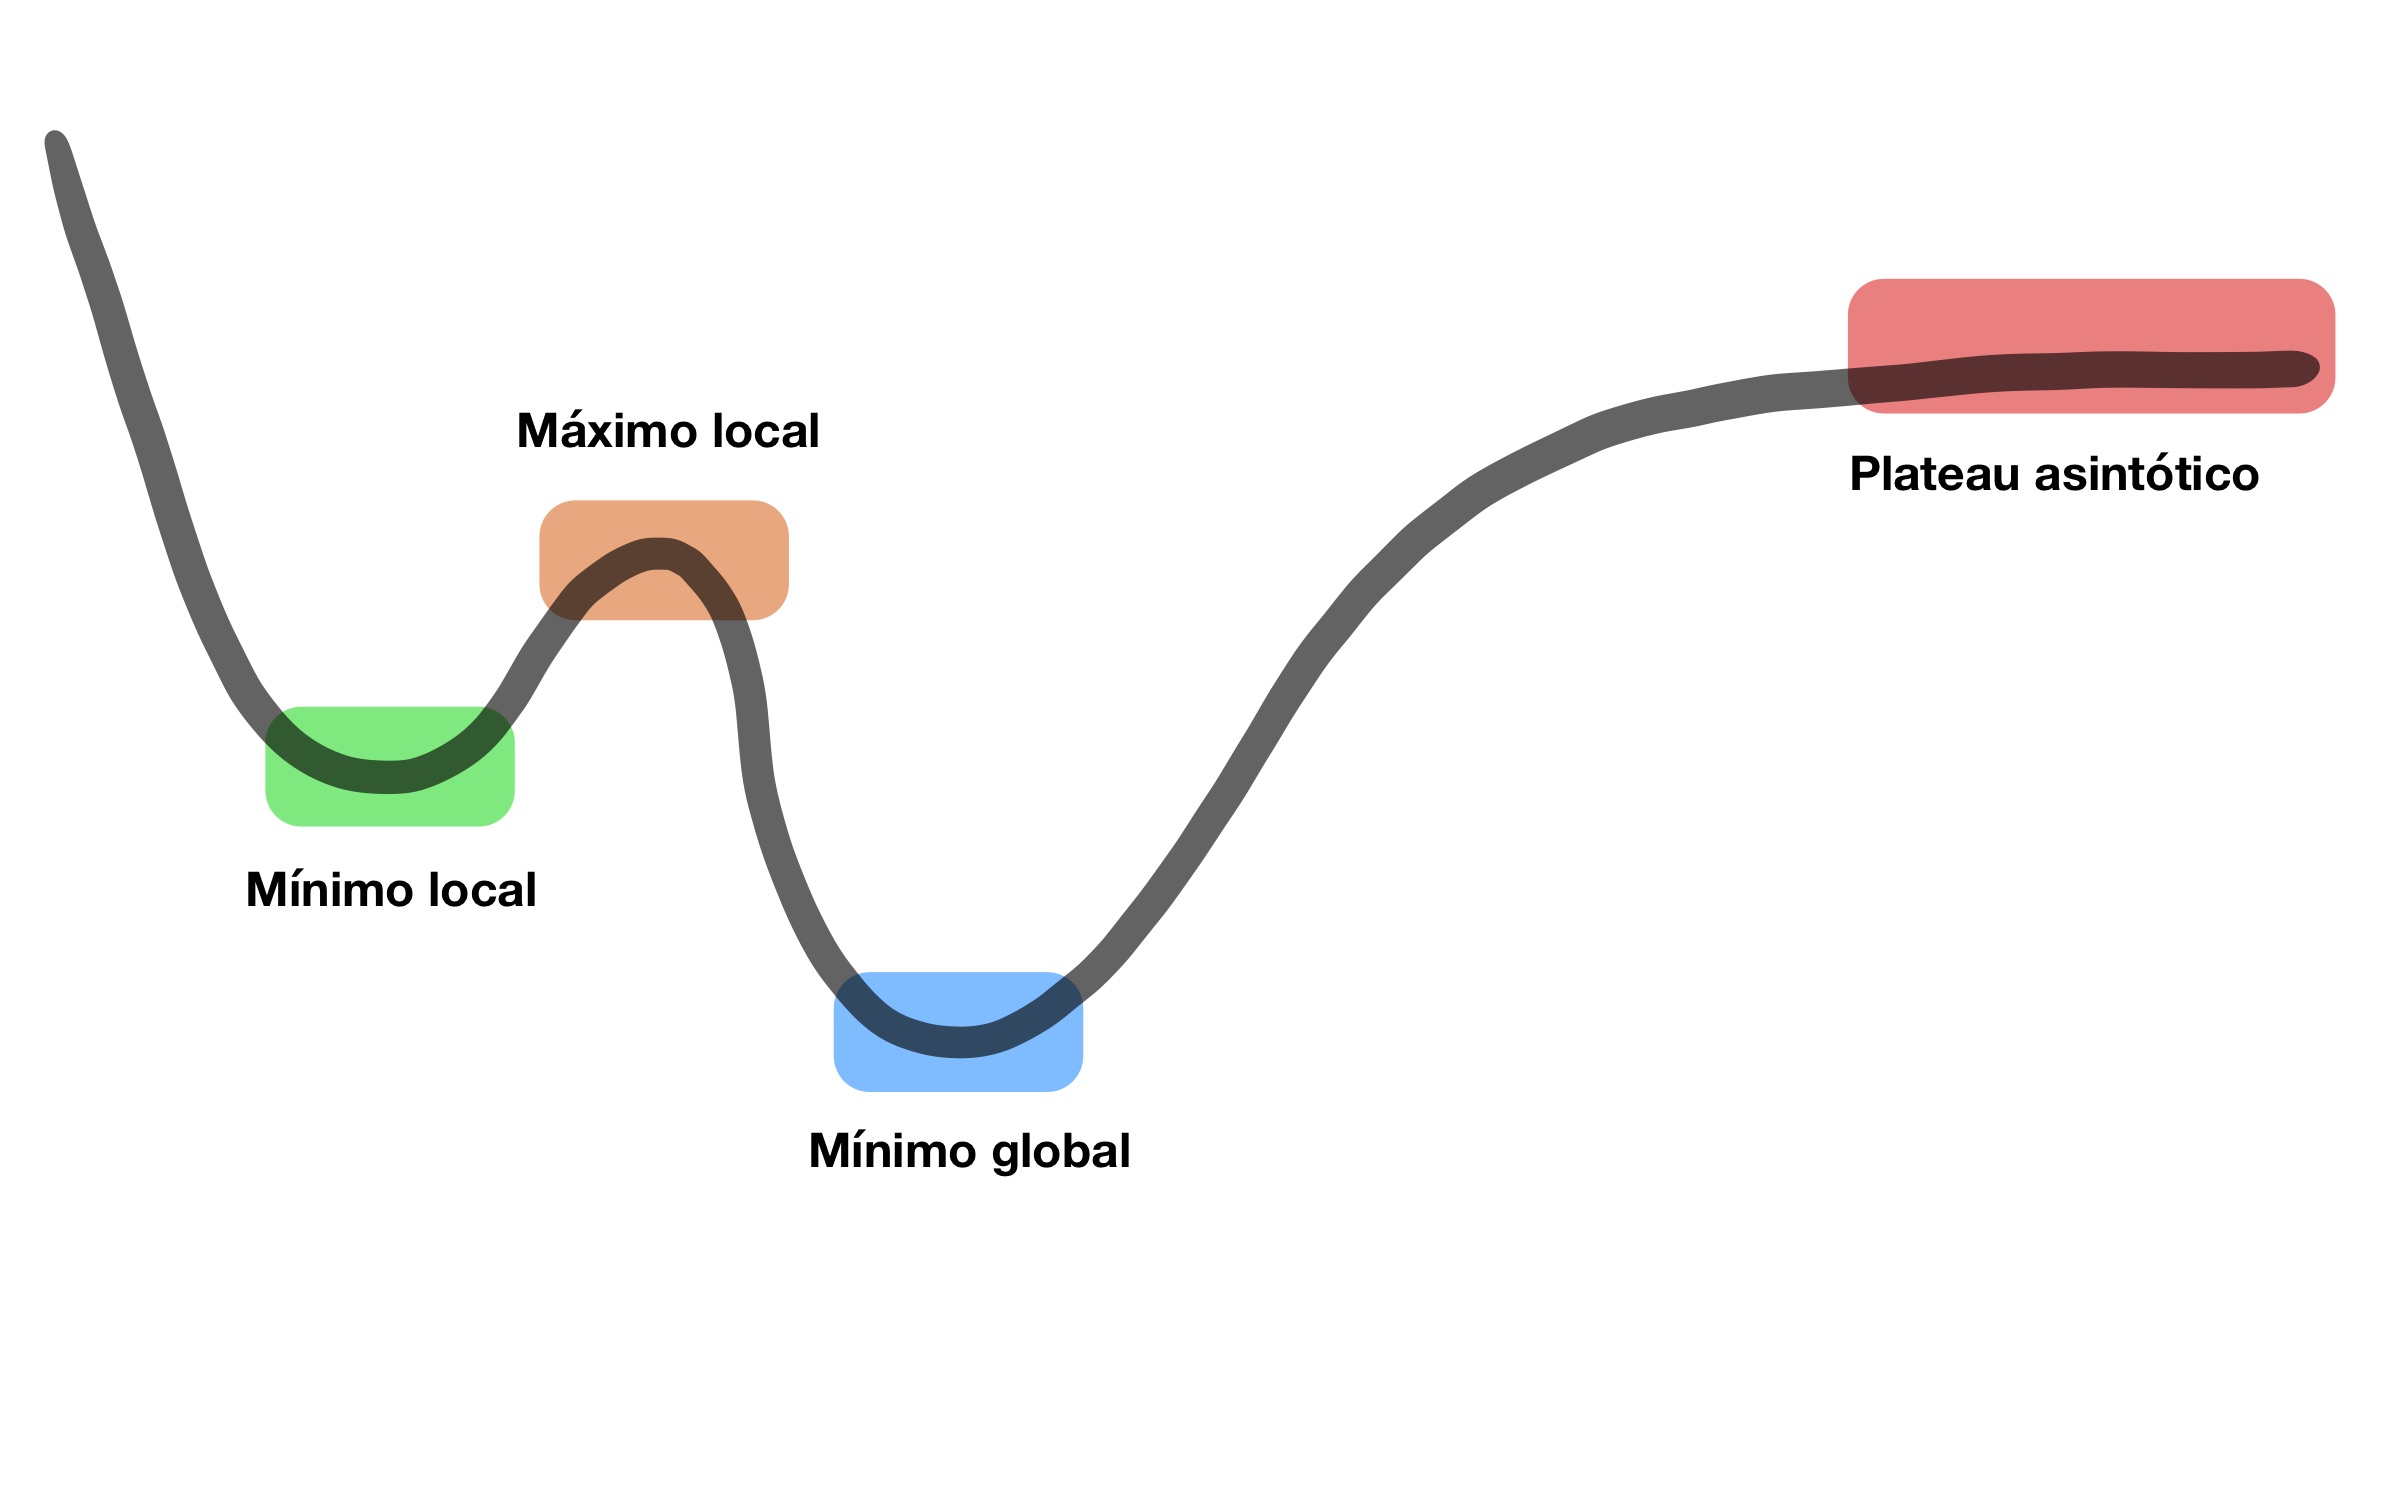
\includegraphics[scale=0.16]{img/Clase_18_pag_09.jpg}
    \caption{Distintos resultados al aplicar S.G.D.}
    \label{fig:sgd}
\end{figure}
% \vspace{1cm}\\
\subsubsection{Tasa de convergencia}
Sobre la tasa de convergencia tenemos las siguientes comparaciones entre descenso de gradiente y descenso de gradiente estocástico:
\newp \textbf{Descenso Gradiente (algoritmo clásico determinista)}
\begin{itemize}
    \item $F$ convexa: $F(\theta_t)-F(\theta^*)=O(\frac{1}{\sqrt{t}})$
    \item Convexa con $\nabla F$ Lipschitz: $F(\theta_t)-\F(\theta^*=O(\frac{1}{t})$
    \item Fuertemente convexa + $\nabla F$ Lipschitz: $F(\theta_t)-F(\theta^*)=O(e^t),\espacio e\in(0,1)$
\end{itemize}
\newp \textbf{Descenso de gradiente estocástico con pasos $\gamma_t\sim \frac{1}{t}$}
\begin{itemize}
    \item $F$ convexa: $F(\theta_t)-F(\theta^*)=O(\frac{1}{\sqrt{t}})$
    \item Convexa con $\nabla F$ Lipschitz: $F(\theta_t)-\F(\theta^*=O(\frac{1}{\sqrt{t}})$
    \item Fuertemente convexa + $\nabla F$ Lipschitz: $F(\theta_t)-F(\theta^*)=O(\frac{1}{t})$
\end{itemize}
\subsection{Variantes de Gradiente Estocástico}
\subsubsection{Gradiente estocástico con Mini-Batch}  % 47:50 clase 18
Es una variante muy utilizada en la práctica. Viene del anglicismo Batch que significa ``lote''.
\newp \textbf{Idea}: en general tenemos
$$ \theta_{t+1}=\theta_t - \gamma_t \partial_\theta f(\theta_t,X_{t+1})=
\theta_t - \gamma_t (\nabla F(\theta_t)+\partial_\theta f(\theta_t,X_{t+1})-\nabla F(\theta_t)\,,$$
donde $\Delta_t=\partial_\theta f(\theta_t,X_{t+1})-\nabla F(\theta_t)$ es aleatorio y lo interpretamos como ruido, con $\E(\Delta_t)=0$. Dicho de otro modo, tenemos un ``gradiente perturbado''.
\newline Notemos que $\partial_\theta f(\theta_t,X_{t+1})$ es un \textbf{estimador insesgado} de $\nabla F(\theta)$. Si tomamos esperanza nos da
$$ \E(\partial_\theta f(\theta_t,X_{t+1}))=\nabla F(\theta_t)\,.$$
Sin embargo también lo es la siguiente expresión, para $m$ fijo:
$$ \displaystyle\frac{1}{m}\sum^m_{i=1}\partial_\theta f(\theta_t,X_{t+i})\,.$$
Más aún, con lo anterior estaremos reduciendo varianza.

\newp \textbf{Descenso de gradiente con mini-batch}:
\newline Sea $m$ fijo (tamaño del mini-batch), y $x_1,\dots,x_t,\dots \iid \sim \mu$, entonces tomamos:
$$ \theta_{t+1}=\theta_t - \gamma_t\cdot \displaystyle\frac{1}{m}\sum^m_{k=1}\partial_\theta f(\theta_t,x_{t+i})$$
con
$$ Var(\displaystyle \frac{1}{m}\sum^m_{k=1}\partial_\theta f(\theta,x_{t+i}))=\frac{Var(\partial_\theta f(\theta,x))}{m}=\frac{\sigma^2}{m}$$
Posee entonces las siguientes ventajas:
\begin{itemize}
    \item El estimador del gradiente posee mucha menos varianza.
    \item Lo anterior implica que hay fluctuaciones más pequeñas.
    \item Aprovecha ``vectorización en computadores'' (GPU, paralelización, ...).
\end{itemize}
\begin{remark}
\beforeitemize
\begin{itemize}
    \item En el caso conexo fuerte con $\gamma_t=\gamma<\frac{2}{\mu}$ se puede probar que
    $$ \E(\|\theta_t-\theta^*\|^2)\leq (1-2 \alpha \mu)^t\|\theta_0-\theta^*\|^2+\frac{\gamma \sigma^2}{m 2\mu}\,,$$
    donde 
    $$ F(\theta)-F(\eta)\geq \nabla F(\theta)(\theta-\eta)+\frac{\mu}{2}\|\theta-\eta\|^2\,.$$
    \item $m$ y $\eta_t$ se deben ajustar conjuntamente.
    \item ``mini-batch'': entre el lote completo de datos (Descenso de gradiente usual) y S.G.D. ``en línea''.
    \item En la práctica, S.G.D. se usa casi siempre con mini-batch, de tamaño fijo $m$ para aprovechar capacidad de cálculo ``paralelo''. El costo de un paso con mini-batch es menor a $m$ por el costo de un paso con un dato.
    \item Tener varianza pequeña no siempre es deseable al comienxo: ayuda a no quedar bloqueado en mínimos locales, por ende tomamos $\gamma_t\searrow$.
    \item Tampoco es necesario ``esperar'' a que las fluctuaciones ``lleguen a $0$'' (con $\gamma_t\to 0$).
    \newline Se puede parar fijando un criterio $|F(\theta_{t_k})-F(\theta_{t_{k+1}})|<\epsilon$\,.
\end{itemize}
\end{remark}

\subsubsection{Más variantes de Gradiente Estocástico}
Existen variantes de descenso de gradiente estocástico que explotan la dinámica determinista subyacente para una convergencia más rápida. Si bien en algunos casos tendremos convergencia, muchas veces estos métodos son heurísticas. Los algoritmos mencionados en esta sección están disponibles en las principales bibliotecas de \textit{python} como \href{https://pytorch.org/docs/stable/optim.html#algorithms}{pytorch}, \href{https://www.tensorflow.org/api_docs/python/tf/keras/optimizers}{tensorflow} y \href{https://mxnet.apache.org/versions/1.7/api/python/docs/tutorials/packages/optimizer/index.html}{Apache MXNet}.
\subsubsubsection{Momentum}
El método momentum utiliza el gradiente de la etapa anterior mediante la siguiente recurrencia:
$$ \theta_{t+1} = \theta_t - \gamma_t m_{t+1} \,,$$
con
$$ m_{t+1}=\beta m_t+(1-\beta)\nabla_\theta f(\theta_t,X_{t+1}), \espacio m_0=0\espacio .$$
Esto mantiene algo de las direcciones de descenso anteriormente usadas (``olvido exponencial'').

\subsubsubsection{AdaGrad}  %1:05
AdaGrad consiste en dividir el paso por un factor proporcional a la norma de los gradientes acumulados hasta entonces.
$$ \theta_{t+1}=\theta_t-\displaystyle \frac{\gamma_t}{\sqrt{v_t+\epsilon}}\nabla_\theta f(\theta,X_{t+1}) \,,$$
para $\epsilon$ fijo y con
$$ v_t = \displaystyle \sum^{t-1}_{k=1}\|\nabla_\theta f(\theta,X_k)\|^2\,,\espacio v_1=0\,.$$
Este método va haciendo que los pasos sean más chicos si hemos dado pasos grandes, evitando salir de buenos mínimos locales. Análogamente, al llegar a una zona plana este factor aumentará, de modo que se pueda salir hacia mejores valores.

\subsubsubsection{Variante Estocástica (Stochastic Gradient Langevin Dynamics)}
La siguiente variante ``agrega estocasticidad'' para explorar de mejor manera el espacio y evitar mínimos locales. Tomamos
$$ \theta_{t+1}=\theta_t-\gamma_t\nabla_\theta f(\theta_t,X_{t+1}) + \beta_t \mathcal{N}_t(0,I_d)\,$$
donde las $ \beta_t\sim \mathcal{N}_t(0,I_d)$ son independientes y representas ruido exógeno. Podemos tomar $\beta_t$ tendiendo a cero (por ejemplo $\beta_t=\sqrt{2\gamma t}$) o bien $\beta_t=\beta$ constante. Con este último, siempre se estará agregando ruido, lo cual puede ser útil para recorrer más el espacio de soluciones.
% \newp Estos temas tienen mucha investigación actual. En particular acerca de algoritmos híbridos entre MCMC y Gradiente Estocástico.

\subsubsubsection{Otras variantes}
Existen más variantes, muchas de las cuales son variantes del método de gradiente determinista adaptadas a gradiente estocástico. Algunas de ellas son:
\begin{enumerate}
    \item RMSprop
    \item NAG (\textit{Nesterov Accelerated Gradient})
    \item AdaDelta
    \item Adam (\textit{Adaptive momentum estimation})
    \item Adamax
\end{enumerate}
Hay teoría que indica cuando podría ser mejor uno u otro. En la práctica se recomienda probar con varios para encontrar la mejor alternativa.

\subsection{Introducción a las Redes Neuronales}
% Motivación.
% \subsubsection{Partes básicas}
% \subsubsubsection{Perceptrón}
% \subsubsubsection{Funciones de activación}
% \subsubsection{Perceptrón}
% \subsubsubsection{Grafo computacional}
Recordemos el Ejemplo \ref{ejemplo:red_neuronal}. Queremos aproximar las etiquetas $y$ usando
% $$ \hat{y}(x,\theta) = \displaystyle \frac{1}{N}\sum^N_{j=1}a_j\sigma(w_j^Tx+b_j) $$
$$ \hat{y}(x,\theta) = \displaystyle \sum^N_{j=1}a_j\sigma(w_j^Tx+b_j) $$
Cada uno de los elementos $\sigma(w_j^Tx+b_j)$ define una función, que se le llama \textbf{perceptrón}. 

\newp El perceptrón tiene una motivación biológica: se inspira de las neuronas biológicas. En una red neuronal combinaremos la acción de varios perceptrones, de modo que la transmisión de información entre un perceptrón y otro simula la sinapsis entre neuronas del cerebro. En este caso, la señal transmitida será numérica, y el que un perceptrón esté o no activado se modelará usando la función de activación $\sigma$, similarmente a como se activaría una neurona. El ejemplo más clásico es una función de activación de Heaviside, que retorna $0$ cuando el input es $\leq 0$ y $1$ en caso contrario.

\newp A la función del ejemplo la llamamos una red de perceptrón de una capa. Analizaremos las capacidades aproximativas de esta arquitectura, que mostramos de manera visual en la figura \ref{fig:MLP}.
\begin{figure}
    \centering
    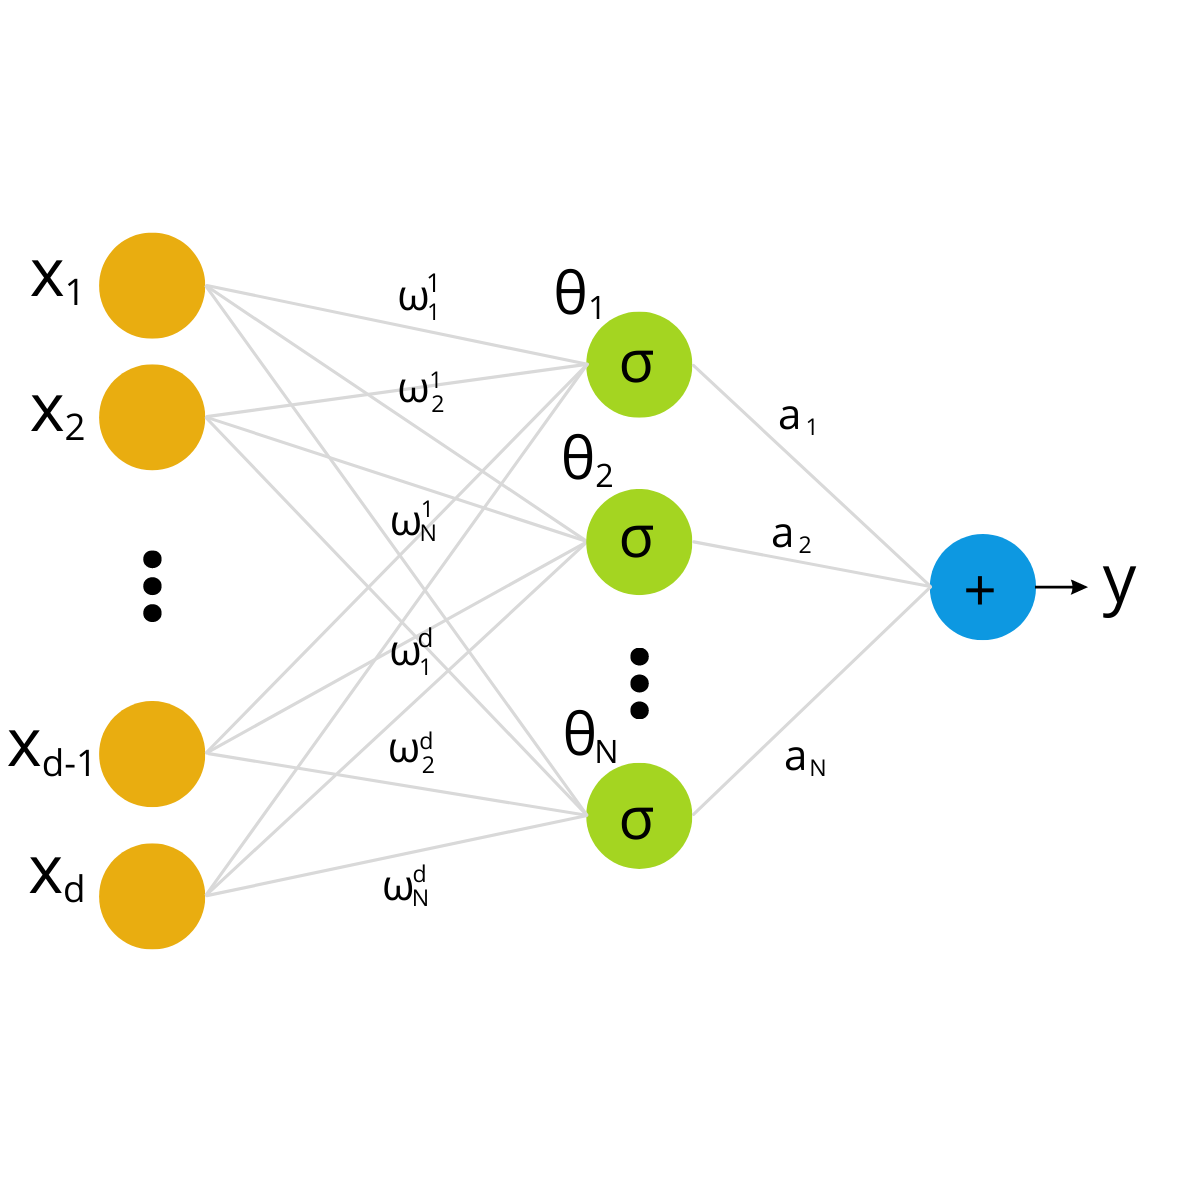
\includegraphics[scale=1.2]{img/MLP.png}
    \caption{Visualización de una red neuronal de una capa}
    \label{fig:MLP}
\end{figure}

% \subsubsection{Aspectos teóricos}
% \subsubsubsection{Teoremas de aproximación universal}
\subsubsection{Teoremas de aproximación universal}
La siguiente subsección está basada en el trabajo de Cybenko (1989) \cite{cybenko}. Para la demostración usaremos elementos de Análisis Funcional, como lo son el Teorema de Hahn-Banach y el Teorema de representación de Riesz. Por otro lado, una versión del mismo resultado demostrado en el mismo periodo por Hornik et al. usa el Teorema de Stone-Weirstrass \cite{hornik}.
\begin{definition}[Función sigmoide]
Decimos que una función $\sigma$ es sigmoide si cumple
$$ \sigma(t) = \begin{cases}
1 & \text{ cuando }t\to\infty \\
0 & \text{ cuando }t\to-\infty
\end{cases}$$
\end{definition}
\begin{example}[Función logística]
A la función $\sigma:\R\mapsto (0,1)$
$$ \sigma(t):= \displaystyle\frac{1}{1+e^{-t}}$$
se le llama función logística. Es el ejemplo más común de una función sigmoide continua.
\\ La activación de Heavisde es también una función sigmoide.
% observacion funcion softmax ???
\end{example}
Asumimos el siguiente resultado sin demostración. Está basado en el uso del teorema de convergencia dominada.
\begin{lemma}
\label{lemma:discrim}
Sea $\sigma$ una función sigmoide, medible y acotada, entonces cumple la siguiente propiedad:
$$ \int_{[0,1]^n}\sigma(y^Tx+\theta)d\mu(x)=0\espacio \forall y\in\R^n,\forall\theta \in\R\espacio \Longrightarrow \espacio  \mu\equiv 0$$
En particular esto es cierto para cualquier función sigmoide continua.
\end{lemma}
\begin{theorem}[Teorema de aproximación universal para activación sigmoide]
\label{teo:AU}
Sea $\sigma$ una función sigmoide continua. Entonces el conjunto de funciones de la forma
$$ G(x) = \displaystyle \sum^N_{j=1}a_j\sigma(w^T_jx+b_j)$$
es denso en $\mathcal{C}([0,1]^n)$, con $\b_j\in\R$, $a_j\in\R\espacio \forall j=1,\dots,N$ y $w_j\in\R^n\espacio\forall j=1,\dots,N$. Dicho de otro modo, para todo $f\in\mathcal{C}([0,1]^n)$ y $\epsilon>0$, $\exists G(x)$ de la forma anterior que cumple
$$ |G(x)-f(x)|<\epsilon\espacio\forall x\in [0,1]^n\,.$$
\end{theorem}
\begin{proof}
\gris
Sea $S\subset\mathcal{C}([0,1]^n)$ el conjunto de las funciones de la forma $\displaystyle \sum^N_{i=j}a_j\sigma(w^T_jx+b_j)$, con  $b_j\in\R$, $a_i\in\R\espacio \forall j=1,\dots,N$ y $w_j\in\R^n\espacio\forall j=1,\dots,N$, y notemos que es un subespacio lineal de $\mathcal{C}([0,1]^n)$. Veamos que $\bar S$ (la cerradura de $S$) es $\mathcal{C}([0,1]^n)$. Por contradicción, si asumimos lo contrario entonces $\bar S$ es un subespacio cerrado propio de $\mathcal{C}([0,1]^n)$. Luego por Hahn-Banach existe un funcional lineal $L$ en $\mathcal{C}([0,1]^n)$, no nulo, pero que se anula en $\bar S$ (y por ende en $S$).

\newp Por el teorema de representación de Riesz, el funcional $L$ debe ser de la forma
$$ L(h) = \displaystyle\int_{[0,1]^n}h(x)d\mu(x)$$
para $\mu$ medida en $[0,1]^n$ y $\forall h\in \mathcal{C}([0,1]^n)$. Luego en particular se cumple que
$$\int_{[0,1]^n}\sigma(y^Tx+\theta)d\mu(x)=0 \espacio \forall y\in\R^n,\forall\theta \in\R$$. Por lema \ref{lemma:discrim}, $\mu\equiv 0$, con lo cual el funcional lineal $L$ es nulo. Como esto es una contradicción, $\bar S = \mathcal{C}([0,1]^n)$, i.e., $S$ es denso en $\mathcal{C}([0,1]^n)$.\findem
\negro
\end{proof}
\begin{remark}
A las funciones que cumplen la propiedad del lema \ref{lemma:discrim} se les llama funciones discriminatorias. El resultado vale entonces para cualquier función discriminatoria continua. Además, se puede generalizar además a funciones sigmoide medibles y funciones sigmoide arbitrarias agregando ciertas restricciones adicionales.

Más aún, existen variados resultados que proponen cotas para el tamaño de la red neuronal dependiendo de la función a aproximar. La versión del Teorema de Aproximación Universal que hemos visto corresponde al caso de ancho arbitrario, donde ancho se refiere a la cantidad de perceptrones de la capa. Análogamente existen versiones de ancho acotado y profundidad arbitraria, donde profundidad se refiere a la cantidad de capas.
\end{remark}
% \begin{remark}[Generalizaciones del Teorema \ref{teo:AU}]
% ...
% \end{remark}

El siguiente resultado nos muestra que el Teorema de aproximación universal nos sirve para implementar un clasificador basado en separaciones del espacio con una red de una sola capa. Primero sea $P_1,\dots,P_k$, $k\in\N$ una partición de $[0,1]^n$, definiremos una función de decisión como un $f:[0,1]^n\mapsto \{1,\dots,k\}$ que cumple
$$ f(x) = j \espacio \ssi \espacio x\in P_j \,.$$
\begin{theorem}
Sea $\sigma$ una función sigmoidal continua. Sea $f$ una función de decisión para alguna partición $\mu$-medible y finita, donde $\mu$ es la medida de Lebesgue en $[0,1]^n$. Para cualquier $\epsilon>0$ existe una suma finita de la forma
$$ G(x) = \displaystyle \sum^N_{j=1}a_j\sigma(w^T_jx+b_j) \,,$$
y un conjunto $D\subset [0,1]^n$ tal que $\mu(D)\geq 1-\epsilon$ y que cumple
$$ |G(x)-f(x)|<\epsilon\espacio \text{ para }x\in D \,.$$
\end{theorem}
\begin{proof}
\gris
Recordemos el Teorema de Lusin, que nos dice que una función finita $\mu$-c.s. es medible si y solo si es una función continua en casi todo su dominio. Luego existe una función continua $h$ y un conjunto $D$ tal que $\mu(D)\geq 1-\epsilon$ de modo que 
$$ h(x)=f(x) \espacio \forall x \in D \,.$$
Como $h$ es continua, por Teorema \ref{teo:AU}, existe una función $G$ de la forma $$G(x)=\displaystyle \sum^N_{i=j}a_j\sigma(w^T_jx+b_j)\,,$$
con  $b_j\in\R$, $a_i\in\R\espacio \forall j=1,\dots,N$ y $w_j\in\R^n\espacio\forall j=1,\dots,N$ que satisface
$$ |G(x)-h(x)|<\epsilon \espacio \forall x\in [0,1]^n\,.$$
Entonces para $x\in D$ tendremos $|G(x)-f(x)|<\epsilon$\,. \findem
\negro
\end{proof}

\subsubsection{Entrenamiento de una red neuronal con Gradiente Estocástico}
Consideremos el caso en el que tengamos una sucesión de $n$ puntos de datos $(x_1,y_1),\dots,(x_n,y_n)\subset \R^d\times\R$. Sea además, $l:\R\times\R\mapsto\R$ una función de error, y denotemos:
$$ \mathcal{L}(\theta) = \displaystyle\frac{1}{N}\sum_{i=1}^n l(y_i,\hat y_i(x_i,\theta)) \,.$$ 
Usaremos el Algoritmo de Descenso de Gradiente Estocástico para minimizar esta función de pérdida. Sin embargo notemos que esto no es tarea fácil, pues involucra el cómputo del gradiente de $\mathcal{L}$, considerando que la dimensionalidad de $\theta$ corresponde al número de parámetros totales de la red neuronal (potencialmente muy grande). Estudiemos como se realiza esto en la práctica.
% \subsubsubsection{Funciones de error}
\subsubsubsection{Cálculo de gradiente con \textit{Back-propagation}}
% \subsubsubsection{Tensores}
Back-Propagation es un algoritmo para calcular derivadas en contextos generales, aunque es principalmente usada en el contexto de redes neuronales. Es particularmente útil cuando tenemos cálculos sucesivos, lo cual es el caso de las redes neuronales, más aún si constan de varias capas de profundidad. Veamos un ejemplo para inspirar su uso.

\newp Sean $\theta$ el conjunto de parámetros de una red neuronal que queremos ajustar. Sabemos que para Gradiente Estocástico tendremos que saber computar el gradiente en un punto para cualquier parámetro en $\theta$. Consideremos una pérdida cuadrática y una aproximación de un dato $y_i$ de la forma
$$ \hat y_i = \displaystyle \sum^N_{j=1} a_j\sigma(\omega^T_j x_i+b_j) $$
Tratemos de calcular la derivada de $l_i=(y_i-\hat y_i)^2$ con respecto a $a_k$, con $k\in\{1,\dots,N\}$:
$$ \frac{\partial l_i}{\partial a_k} = \frac{\partial (y_i-\hat y_i)^2}{\partial a_k} = 2(y_i-\hat y_i) \frac{\partial (y_i-\hat y_i)}{\partial a_k} \,.$$
Notemos que hasta este punto, sólo usamos la regla de la cadena. Ahora como $y_i$ es un punto fijo de dato que no depende de $a_k$, nos queda:
$$ \frac{\partial l_i}{\partial a_k} = 2(y_i-\hat y_i) \frac{\partial (y_i-\hat y_i)}{\partial a_k} =  -2(y_i-\hat y_i) \frac{\partial\hat y_i}{\partial a_k} =  -2(y_i-\hat y_i) \frac{\partial[\sum^N_{j=1} a_j\sigma(\omega^T_j x_i+b_j)]}{\partial a_k} = -2(y_i-\hat y_i)\sigma(\omega_k^Tx_i+b_k)$$
Denotaremos ahora las variables auxiliares siguientes. El objetivo será simplificar lo anterior:
\begin{itemize}
    % \item $l_i = l(y_i,\hat y_i)$
    \item $z_i = (y_i-\hat y_i)$
    \item $u^j_i = a_j\sigma(\omega^T_j x_i+b_j)$
    \item $v^j_i = \omega^T_j x_i+b_j$
\end{itemize}
Podemos reescribir el cálculo de la última linea usando las variables auxiliares:
$$ \frac{\partial l_i}{\partial a_k} = 2(y_i-\hat y_i) \frac{\partial[\sum^N_{j=1} a_j\sigma(\omega^T_j x_i+b_j)]}{\partial a_k} = 2z_i \frac{\partial[\sum^N_{j=1} u^j_i]}{\partial a_k} = 2z_i \frac{\partial u_i^k}{\partial a_k} \,.$$
En este punto podemos notar que 
$$ \frac{\partial u_i^k}{\partial a_k} = \frac{\partial[a_k \sigma(v_i^j)]}{\partial a_k} = \sigma(v_i^j) \espacio \therefore \espacio \frac{\partial l_i}{\partial a_k}=2z_i \sigma(v_i^j)$$
Si bien agregar las variables auxiliares nos hace pesada la notación, la idea es guardar la información paso por paso a medida que los valores ``avanzan'' en la red neuronal hasta llegar a la predicción. Esto a la larga será útil, pues se nos facilitan los cálculos, como vimos en derivar $\frac{\partial l_i}{\partial a_k}$. Por otro lado notemos que podemos llegar a $l_i$ de manera acumulativa desde los parámetros usando las variables auxiliares.
\begin{itemize}
    \item $l_i = z_i^2$
    \item $z_i = (y_i-\sum^N_{j=1}u_i^j)$
    \item $u^j_i = a_j\sigma(v_i^j)$
    \item $v_i^j = \omega^T_j x_i+b_j$
\end{itemize}
Luego usando la regla de la cadena podemos deducir que
$$ \frac{\partial l_i}{\partial a_k} = \frac{\partial l_i}{\partial z_i}\frac{\partial z_i}{\partial u_i^j}\frac{\partial u_i^j}{\partial a_k} = 2z_i \cdot 1 \cdot \sigma(v_i^j) \,$$
i.e., hicimos el mismo cálculo anterior pero basado en cálculos simples de derivadas usando las variables auxiliares. Veamos otro ejemplo. Calcularemos $\frac{\partial l_i}{\partial b_k}$ usando este principio:
$$ \frac{\partial l_i}{\partial b_k} = \frac{\partial l_i}{\partial z_i}\frac{\partial z_i}{\partial u_i^j}\frac{\partial u_i^j}{\partial v_i^j}\frac{\partial v_i^j}{\partial b_k} = 2z_i \cdot 1 \cdot a_k\sigma'(v_i^j)\cdot 1 = 2 (y_i-\sum^N_{j=1}u_i^j)a_k\sigma'(\omega^T_j x_i+b_j) \,$$
donde $\sigma'$ es la derivada de la función de activación $\sigma$ (unidimensional). \newp Notemos la facilidad con la que llegamos a la expresión final, y más aún, notemos que muchas de las derivadas parciales que usamos también se usaron para computar $\frac{\partial l_i}{\partial a_k}$. Se puede hacer un cálculo análogo para llegar a $\frac{\partial l_i}{\partial \omega_k}$, con lo cual tendríamos calculado el gradiente de $l_i$. 
\newp El algoritmo Back-Propagation consiste en el uso exhaustivo de la \textbf{regla de la cadena}. Calculamos derivadas parciales paso por paso y las guardamos para usarlos en cada parámetro. De este modo que sólo computaremos derivadas simples y guardarlos evitará hacer cálculos redundantes. %La única restricción que tenemos para usar Back-Propagation es que no hayan cálculos circulares.
En nuestro caso no era imposible calcular el gradiente, pero a medida que las redes neuronales sean más profundas, más profundas serán las dependencias entre variables y por ende más cálculos se ahorrarán si usamos regla de la cadena, además de simplificar el computo.

\newp Las bibliotecas que implementan redes neuronales, como \textit{pytorch} implementan este algoritmo implícitamente, de modo que al definir las operaciones entre variables, se guardan las derivadas parciales respectivas. Durante el entrenamiento, una vez que la información pasa a través de la red neuronal para computar una predicción, se computará un error (\textit{forward}). Enseguida, se computa el gradiente usando las operaciones que estaban guardadas, haciendo fluir la información en reversa hasta tener el valor de cada derivada parcial (\textit{backward}). Esto nos da una manera eficiente de usar descenso de gradiente estocástico.

\subsubsubsection{Problemas y prácticas usuales}
% El uso de redes neuronales ha ido evolucionando con el tiempo. Muchas de las innovaciones son resultado de experimentos que han funcionado bien en la práctica.
Hasta ahora hemos observado las capacidades teóricas de las redes neuronales de una sola capa. Si bien poder aproximar funciones continuas parece una capacidad muy valiosa, no siempre estaremos intentando aproximar funciones con buenas propiedades. Es más, muchas veces no tendremos ninguna garantía de que las funciones que estamos tratando de aproximar existan. Tener un cierto grado de profundidad nos ayuda a aumentar el poder de expresividad de los valores de salida. A su vez podremos disminuir el número de perceptrones en cada capa.
% figura
\newp Lamentablemente, un problema que se encuentra al entrenar redes neuronales profundas es el \textbf{desvanecimiento del gradiente}. Esto sucede cuando el valor de las derivadas parciales es pequeño, evitando que puedan actualizarse valores de capas iniciales usando descenso de gradiente. Dentro de las soluciones que se han explorado para evitar este problema está el uso de la función de activación \textit{ReLU} (\textit{rectified linear unit}), que está dada por:
$$ ReLU(t) = \begin{cases}
t & \text{ cuando }t\geq0 \\
0 & \text{ cuando }t<0
\end{cases}$$
Si bien esta función no es sigmoide y es no-acotada, es mucho más fácil de computar, es invariante a la escala. El problema de que no sea derivable en $0$ se arregla simplemente asignando $1$ o $0$ como valor de la derivada en aquel punto. Por último notar que podemos lograr funciones que si son sigmoides al acoplar dos funciones \textit{ReLU} o más. Un ejemplo de esto es la función $\sigma$ siguiente:
$$ \sigma(t) = \frac{1}{2}(ReLU(t+1)-1-(ReLU(t-1)-1))\,,$$
que es una función sigmoide continua, y por ende cumple con las hipótesis del Teorema \ref{teo:AU}. En la figura \ref{fig:fun_activ} se muestran algunas de las funciones de activación que se han mencionado en esta subsección.
\begin{images}[\label{fig:fun_activ}]{Ejemplos de funciones de activación}
	\addimage{RRNN_escalon}{width=6.5cm}{Activación de Heaviside}
	\addimage{RRNN_logistic}{width=6.5cm}{Logística}
	\imagesnewline
	\addimage{RRNN_ReLU}{width=6.5cm}{$ReLU(t)$}
	\addimage{RRNN_two_ReLUs}{width=6.5cm}{$\frac{1}{2}(ReLU(t+1)-1-(ReLU(t-1)-1))$}
\end{images}


% \subsubsection{Otros tipos de redes neuronales}
% \subsubsubsection{Redes convolucionales}
% \subsubsubsection{Redes recurrentes}

% \subsubsection{Aplicaciones en matemáticas}
